\documentclass{beamer}
\usepackage{graphicx}
\usepackage{amsmath}

\newcommand{\R}{\mathbb{R}}
\newcommand{\N}{\mathbb{N}}
\newcommand{\Z}{\mathbb{Z}}
\newcommand{\Q}{\mathbb{Q}}
\newcommand{\C}{\mathbb{C}}
\newcommand{\F}{\mathbb{F}}

\begin{document}

\title{Proving Gauss's Lemma in Lean}

\author{Aditya Agarwal}

\institute{Australian National University}

\date{\today}

\begin{frame}
  \titlepage
\end{frame}

% I should note that this is the polynomial lemma. 

\begin{frame}{Outline}
  \tableofcontents
\end{frame}

\section {Lean}

\begin{frame}{What is Lean?} 
    \begin{itemize}
        \item Lean is an Automated/Interactive theorem prover.
        \item Other examples include HOL and Coq.
        % \item Can be for programming/assertions/metaprogramming etc. but we mainly use it for writing proofs.
        \item You encode proofs in a formal language and Lean checks it's correctness
        \item Lean can also infer some of the details of the proof for you.
    \end{itemize}         
\end{frame}

\begin{frame}{Proofs in Lean} 
  There are two ways of writing proofs in Lean, Term mode and Tactic mode. 

\end{frame}


\begin{frame}{Term Mode} 

  In term mode you explicitly write down every step of the proof. 

  \

  Example:

  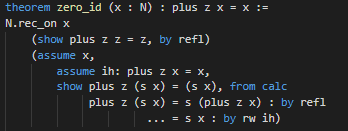
\includegraphics{term_example.png}

\end{frame}

\begin{frame}{Tactics  Mode} 

  Tactics mode allows you to use ``tactics'', which direct Lean on how it should work towards the next step.

  \

%  This can lead to marvellously opaque proofs, where you just chain tactics.  
  Example:

  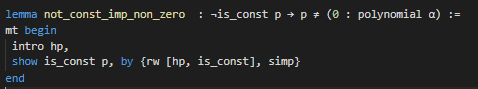
\includegraphics{tactics_example.png}

  %  You can jump between the proofs anytime
\end{frame}



\section {Dependent Type Theory}

\begin{frame}{Dependent Type Theory}
  % Lean does not use the standard ZFC construction of mathematics under the hood. 

  Lean is built on Dependent Type Theory, an alternative foundation of mathematics. Specifically, it implements the Calculus of Inductive Constructions.
\end{frame}

\begin{frame}{Dependent Type Theory}
  % I won't go too much into detail because it is another presentation in itself, but
  \begin{itemize}
    \item Each object has a type. 
    \item E.g. 
      \begin{itemize}
        \item $n : \N$
        \item $p \iff  p : Prop$
      \end{itemize}

    \item This type may depend on a parameter such as 
    
    \begin{itemize}
      \item $\text{list } \alpha$
      \item $\text{polynomial } \alpha$
    \end{itemize}

    % There is a bit more about Pi types - which depend on a function argument and Sigma types which generalise the cartesian product and so on. 

    % The most important point to not is that

    \item The type of this object is fixed %, and cannot be changed. We might want to say n is a natural number, so it is also a rational number. But Lean does not allow that. 

    % Another thing worth noting is that Lean subscribes to a constructive form of mathematics. So we do not have the Law of the Excluded Middle or Axiom of Choice by default. However, we can work around it by explicitly specifying that we are using classical logic, and my marking any sections where we use choice as non-computable. 

  \end{itemize}

\end{frame}


\section {mathlib}

\begin{frame}{Mathlib}

  Mathlib is the mathematical components library for Lean. 
  \begin{itemize}
    \item It contains the very beginnings of Algebra, Analysis, Topology, and Category Theory. 
    \item On the Algebra side, it contains basic definitions about Groups, Rings, Modules etc. 
    \item And properties about Integral Domains, Euclidean Domains, Unique Factorisation Domains etc. 
    \item Galois Theory is missing entirely.  
  \end{itemize}

  % So I chose to implement Galois Theory. The First Step in which was proving the Gauss Lemma.

\end{frame}

\begin{frame}{Mathlib}
  Generally, mathlib implements theories in the most abstract setting possible. 

  For example, polynomial is defined as

  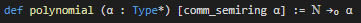
\includegraphics{polynomial.png}

  \begin{itemize}
    \item  This is motivated by the desire for code reuse. 
    \item E.g. We know that any ordered finite set has a maximum. This property can be used wherever ordered finsets come up. 
          like to argue that there is a coefficient of maximum degree. 
    \item Alternative implementations like lists of coefficients would require a separate proof about the fact. 
    \item Similarly, it provides a uniform API between components of the library. 
    \item However, this does have the disadvantage that definitions can become non-intuitive.
  \end{itemize}
\end{frame}

\section {Gauss's Lemma}

\begin{frame}{Gauss's Lemma}
  \begin{theorem}
    Let $\alpha$ be a Unique Factorisation Domain. 

    Let $p$ be a polynomial with coefficients in $\alpha$. Then $p$ factors in $\alpha[X]$ if and only if it factors in $Frac(\alpha)[X]$.
  \end{theorem}
\end{frame} 

\begin{frame}{Gauss's Lemma}
  \begin{definition}
    Let $p$ be a polynomial. We say $p$ is primitive if the only constants in $ \alpha $ which divide $p$ are units. 
  \end{definition}

  \begin{lemma}[Gauss's Primitive Polynomial Lemma]
    Let $p,q$ be primitive polynomials. Then $pq$ is a primitive polynomial.
  \end{lemma}

\end{frame}

\begin{frame}{Gauss's Primitive polynomial Lemma}
  \begin{proof}
    Assume for a contradiction that $pq$ is not primitive. 
    Then we have some $c \in \alpha$ such that $c$ is not a unit and $c \mid p$. 
   
    $\alpha$ is a UFD, so $c$ has some irreducible factor that divides $pq$. So WLOG, we may assume $c$ is irreducible, and hence prime.

    $\therefore \alpha/(c)$ is a domain.
    
    $\therefore \alpha/(c) [x]$ is a domain. 

    $c \mid pq$ so $pq$ vanishes in $\alpha/(c) [x]$. 

    As $\alpha/(c) [x]$ Integral Domain, $p$ vanishes or $q$ vanishes.

   $\therefore c \mid p$ or $c \mid q$. 
    
   $\therefore$ Either $p$ or $q$ is not primitive. 

   Contradiction.
  \end{proof}

\end{frame}

\begin{frame}{Gauss's Lemma {($\implies$)}}

  \begin{proof}

    Let $p$ be an irreducible in $\alpha$. Any irreducible term must be primitive, so we know $p$ is primitive. 

    Suppose for a contradiction that $p$ is not irreducible in $Frac (\alpha)$. 

    Then $p = ab$, for some $a,b \in Frac (\alpha)[x]$. 

    We may multiply $a$ and $b$ by some $c_1,c_2 \alpha$ so that $c_1a,c_2b$ have $\alpha$ coefficients. $c_1c_2p = c_1ac_2b$. 
    We can factor $c_1a$ to some $c_1'a'$ and $c_2b$ to $c_2'b'$, so that $a'$ and $b'$ are primitive. 


  \end{proof}
  
\end{frame}

\begin{frame}
  \begin{proof} (contd.)
    
    Hence $p = \frac{c_1'c_2'}{c_1c_2}a'b'$.

    If $\frac{c_1'c_2'}{c_1c_2}$ in $\alpha$, then we have produced a factorisation for $p$. A contradiction. 

    If $\frac{c_1'c_2'}{c_1c_2}$ is not a unit in $\alpha$, then the denominator in reduced form of $\frac{c_1'c_2'}{c_1c_2}$ must divide each coefficient of $a'b'$, because $p =  \frac{c_1'c_2'}{c_1c_2}a'b'$ has $\alpha$ coefficients. 
  
    Hence $a'b'$ is not primitive. Contradiction.

  \end{proof}
  
\end{frame}

\section{The Proof in Lean}

\begin{frame}{Proof in Lean}
  I took two broad approaches towards implementing the proof in Lean. 

  \begin{itemize}
    \item Proof Above 
    \item A proof using the notion of content. 
  \end{itemize}

  The content is defined as the ideal generated by all the coefficients of $p$. 
  
  The content proof is broadly similar to the proof above, but by using properties of Ideals, it avoids the need for Unique Factorisation (Just the presence of a GCD). 

  However, Lean doesn't have a decent API for dealing with $R$-linear combinations, so I abandoned it. 

\end{frame}


\begin{frame}{Defining the Lemma}

  \begin{theorem}
    Let $p$ be a polynomial with coefficients in $\alpha$. Then $p$ factors in $\alpha[X]$ if and only if it factors in $Frac(\alpha)[X]$.
  \end{theorem}

  \begin{itemize}
    \item $p$ is a polynomial with coefficients in $\alpha$, i.e. of type $\texttt{polynomial } \alpha$. 
    \item Factorisation in $Frac(\alpha)[X]$ only makes sense for polynomials in \texttt{polynomial (quotient\_ring} $ \alpha\texttt{)}$. 
    \item So we explicitly need to specify that the canonical embedding of $p$ is irreducible. 
  \end{itemize}

  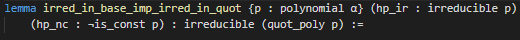
\includegraphics[width=\textwidth]{gauss_fwd.png}
  
\end{frame}

\begin{frame}{Rationals that are Integers}
  % Explicitly specifying that the obvious embedding of $p$ in $Frac \alpha$ is irreducible isn't too bad. 

  \begin{itemize}
    \item  Similarly, we cannot claim that an element of $Frac\ \alpha$ is an element of $\alpha$. 
    \item Lean only has total functions, so we cannot define any \texttt{to\_base:} $Frac\ \alpha \rightarrow \alpha$ directly. 
    \item We may use an option type, defining 

    \texttt{to\_base:} $Frac\ \alpha \rightarrow \texttt{option } \alpha$. 

    An option type is a wrapper around alpha, so f(a) may be Just a or Nothing. 


    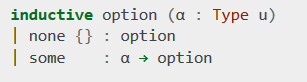
\includegraphics[]{option.png}

  \end{itemize}

\end{frame}

\begin{frame}
  \begin{itemize}
    \item We may choose to define a coercion that depends on a hypothesis that somehow guarantees that the function is well defined. 
    \item But dealing with options or carrying additional hypotheses around around would get annoying very quickly.
    \item So I chose to account for a rational $r$ being an integer by stating 
    $\exists(a : \alpha), \texttt{to\_quot } a = r$. 

    This does have the disadvantage that I have additional variables to worry about. 

    So, for example, so state that a scalar multiple of $m$ is an $@alpha$ polynomial, I wrote the following:

    
\includegraphics[width=\textwidth]{exists.png}


    % But on the balance I figured that would be the least annoying option. 
  \end{itemize}

\end{frame}

\begin{frame}{The Actual Proof}
    The source code is up on GitHub, at \url{https://github.com/chocolatier/theoremproving/}. 
    
    Keeping the above points in mind, it is quite straightforward. 
\end{frame}

\end{document}

